\documentclass[11pt, a4paper]{article}
\usepackage{graphicx, fullpage, hyperref, listings}
\usepackage{appendix, pdfpages, color}

\usepackage{tocloft}            % This squashes the Table of Contents a bit
\setlength\cftbeforesecskip{3pt}

\definecolor{MyLightYellow}{cmyk}{0,0.,0.2,0}

\setlength{\parskip}{4pt}        % sets spacing between paragraphs
\interfootnotelinepenalty=500    % this prevents footnotes breaking across pages

\title{
\includegraphics[width=0.4\textwidth]{UnivCrest}
        \\Experiment 22 - Monte Carlo Simulation}          % <<<<<<<<< change the title as appropriate
\author{%\textcolor{red}{Student ID 200123456 (Group 999)}                % <<<<<<<<< your ID and group number
        \\  \textcolor{red}{ELEC273}\footnote{\textcolor{red}{IMPORTANT: In a standard technical report, you would need to include here your personal details as the author of the document. However, remember that marking of coursework is anonymous and therefore you should remove this part before submitting your report for Year 2 labs! Do not include your name, student ID, email address or any other personal information.}}}                                    % <<<<<<<<< module code
\date{\tiny{\today}}

\begin{document}
\begin{titlepage}
\maketitle
\addtocontents{toc}{\protect\thispagestyle{empty}} % because we don't want a page number on the title page
                                                   % Thanks to Huang Shanyue for suggesting this

\begin{abstract}
This report introduced the results and discussion of the experiment which aiming to explore the features and applications of Monte Carlo method. A penalty kicking model was established wit Matlab with random kicks following uniform distribution and Gaussian distribution. The situation with no goalkeeper, uniformly acted goalkeeper and goalkeeper with special strategy were considered. In the discussion section, the pro and con of Monte Carlo method, the influence of changing of standard deviation in Gaussian cases, and some possible suggestions for penalty kicks participants were studied.
\end{abstract}

\fbox{
\begin{minipage}{0.9\linewidth} \footnotesize
\begin{center} \textbf{Declaration} \end{center}
I confirm that I have read and understood the University's definitions of plagiarism and collusion from the Code of Practice on Assessment. I confirm that I have neither committed plagiarism in the completion of this work nor have I colluded with ant other party in the preparation and production of this work. The work presented here is my own and in my own words except where I have clearly indicated and acknowledged that I have quoted or used figures from published or unpublished sources (including the web). I understand the consequences of engaging in plagiarism and collusion as described in the Code of Practice on Assessment (Appendix L).
\end{minipage}
}

\thispagestyle{empty}
\newpage
\tableofcontents
\end{titlepage}


%-------------------------------------------------------------------------------------------------------
\section{Introduction}
%-------------------------------------------------------------------------------------------------------

Monte Carlo method was a method to solve problems that can be transformed to statistical problems. The theory of Monte Carlo method is to utilize random variables to simulate statistic problems and apply means to approach the theoretical result. This method was first put forwarded by scientists who worked for producing the first nuclear weapon in the world. The Monte Carlo method introduce procedures to simulate a realistic problem step by step. The first step is to design a set of random samples of size N from according probability distribution methods. Secondly, obtain the values of this part by implementing respective methods. Thirdly, calculate the value wanted from this set of samples. Fourthly, repeat the above steps for R times and examine the actual value with these partial results. \cite{ref:lab}

Monte Carlo method was widely used in physics, computing Science, finance, telecommunications and games etc.. With the development of computer technology, the effective and efficiency of the application of Monte Carlo method were considerably improved, which indicated more general value of this method for modern industry. It was significant to explore and acknowledge some basic features and usages of Monte Carlo method.


%-------------------------------------------------------------------------------------------------------
\section{Materials and Methods}
%-------------------------------------------------------------------------------------------------------



To easily simulate penalty kicks events, a simple goal model was established according to the instruction on the lab script\cite{ref:lab}. In this experiment, Matlab was utilized to modeling the situation with pseudo random number generated with Monte Carlo algorithm.


\begin{figure}[htbp]     \begin{centering}
    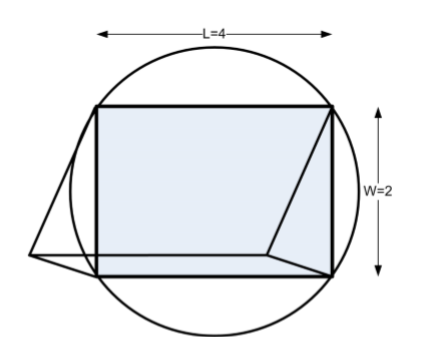
\includegraphics[width=0.5\textwidth]{goal.png}
    \caption{Goal Model (taken from~\cite{ref:lab})}
    \label{Fig:goal}
    \end{centering}
\end{figure}


It is assumed that the ball can be kicked randomly and will only fall in the circle area as it shown in Figure \ref{Fig:goal}. The distribution of balls is expected to follow certain distribution model, such as uniform distribution and normal distribution. In order to explore the distinctions between among different distribution models under diverse conditions, this experiment was designed into two parts. The first part was for the situation with no goalkeepers while the second part focused on the condition that the goalkeeper acted.

\subsection{Part 1: No Goalkeeper Tests}

In this part, the situation with no goalkeeper was modeled. Firstly, the theoretical result of the hit rate was calculated under the assumption that the distribution of balls follows uniform distribution. Secondly, Matlab was utilized to simulate this process with a uniform random number generator. Thirdly, the influence of simulating shots number N and experiment repeat times R was studied with perspectives of line charts generated with Matlab. Furthermore, the hypothesis was changed to that the distribution of balls abides by Gaussian distribution and the experiment steps above were repeated for this new assumption.

\subsection{Part 2: With Goalkeeper Tests}

\begin{figure}[htbp]     \begin{centering}
    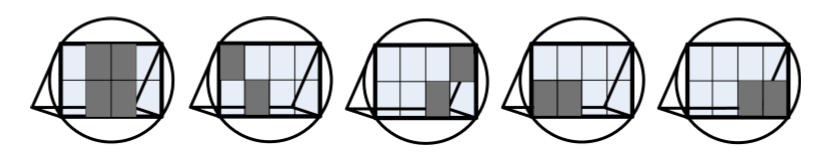
\includegraphics[width=0.5\textwidth]{goalkeeper-action.png}
    \caption{Goalkeeper Action to Penalty Shoot-outs (taken from~\cite{ref:lab})}
    \label{Fig:goalkeeper-action}
    \end{centering}
\end{figure}

Under the condition that there are goalkeeper, this football goal model can be further improved. To easily analyse the situations, the action of the goalkeeper was classified into five types ideally, as shown in Figure \ref{Fig:goalkeeper-action}. Firstly, it was considered that the possibility of these five cases was equal following uniform random distribution. Matlab was used to simulate the shooting process and then the hit rate can be figured out. Secondly, similarly with the produce in Part 1, the hypothesis was changed from uniform random distribution to Gaussian random distribution and the simulation was implemented again. Thirdly, the actions of goalkeeper was updated from equally distributed to that 90\% of the time the goalkeeper may choose position 4 and position 5. Under this circumstance, the probability of scoring was required to be simulated with kicking 100 and 1000 balls.



% You may want to use the {enumerate} environment for a numbered list.
%
%\begin{enumerate}
%    \item First numbered item
%        \subitem You can even have nested layers
%    \item Second numbered item
%    \item Third numbered item
%\end{enumerate}


%-------------------------------------------------------------------------------------------------------
\section{Results}
%-------------------------------------------------------------------------------------------------------

\subsection{Part 1: No Goalkeeper Tests}

This section presents and comments the result from the simulation with no goalkeeper.

\subsubsection{Task 1: Calculation}

In this subsection, the theoretical value of scoring probability will be calculated under the condition that balls distributed in the circle with a radius of $\sqrt{5}$ (as shown in Figure \ref{Fig:goal}) uniformly. In this case, the hit rate can be obtained through the fraction of the goal area and the circle area presented in Equation \ref{eq:posibility_by_area}.

\begin{equation}
P_{scoring} = \frac{S_{rect}}{S_{circle}}.
\label{eq:posibility_by_area}
\end{equation}

As the area of the rectangle goal is $8$ and the area of the circle zone is $5\pi$, the possibility then can be computed, which is 51.0\%.


\subsubsection{Task 2\&3: Matlab Simulation}

To simulate a uniform random kicking situation, Matlab was utilized to generate virtual kicking and display the distribution in illustration. The code was shown in Listing \ref{sct2} in Appendix. This code achieved the requirement of both Task 2 and Task 3, which allowed user to input the shots times N and experiment repeat times R and then the possibility of scoring would be given out and a illustration of shotting will be presented.

\begin{figure}[htbp]     \begin{centering}
    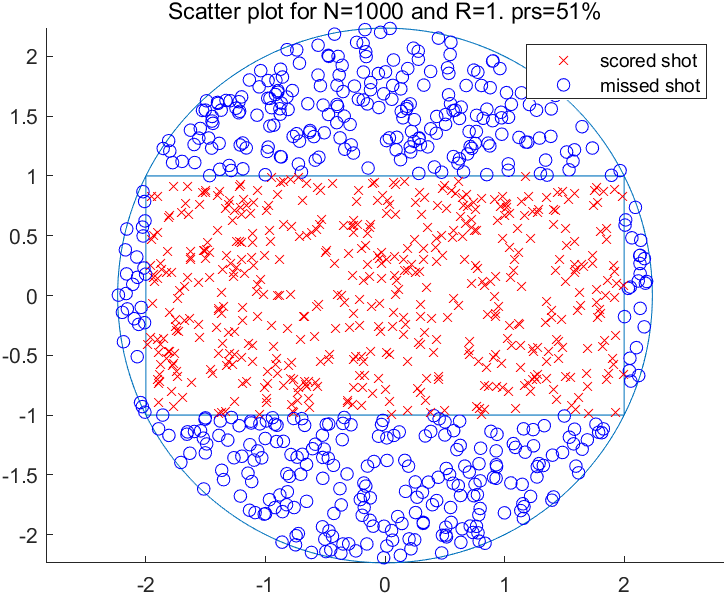
\includegraphics[width=0.5\textwidth]{img/t3.png}
    \caption{Shotting Illustration with N=1000 \& R=1 (Task 3)}
    \label{Fig:task3}
    \end{centering}
\end{figure}


Run the code, with the input of $N=1000$ and $R=1$, it was indicated that the scoring possibility was approximate 51\% and the generated shotting illustration was shown in Figure \ref{Fig:task3}.

\subsubsection{Task 4: Perspective Towards N}

\begin{figure}[htbp]     \begin{centering}
    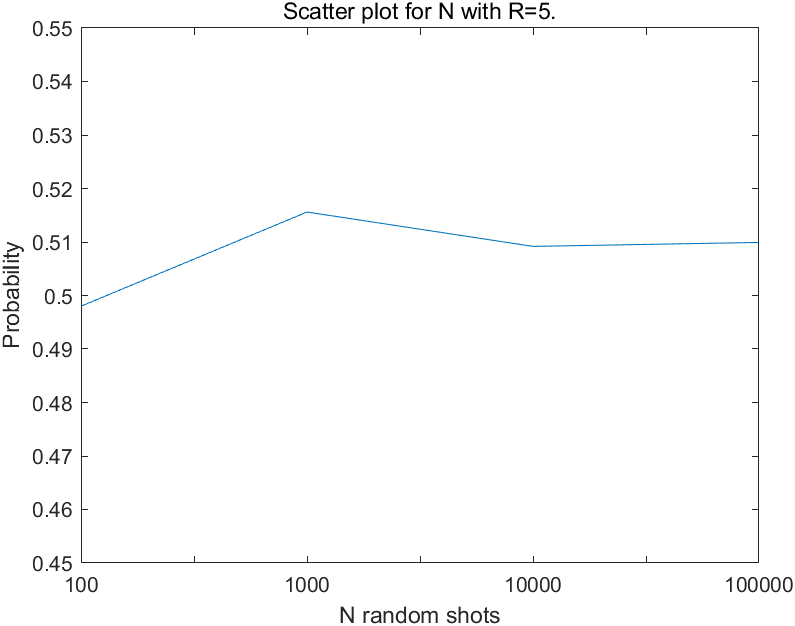
\includegraphics[width=0.5\textwidth]{img/t4.png}
    \caption{Line Chart of Probability against N with R=5 (Task 4)}
    \label{Fig:task4}
    \end{centering}
\end{figure}

With the code in Listing \ref{sct4}, a line chart of scoring probability against N can be obtained. As it presented in Figure \ref{Fig:task4}, the value of the probability approached 51\% when the N increased. This may indicate that, with the shotting times increasing, the experimental value could become more stable and approach the theoretical value, which is 51.0\% as it mentioned in Task 1 in this case.


\subsubsection{Task 5: Perspective Towards R}

\begin{figure}[htbp]     \begin{centering}
    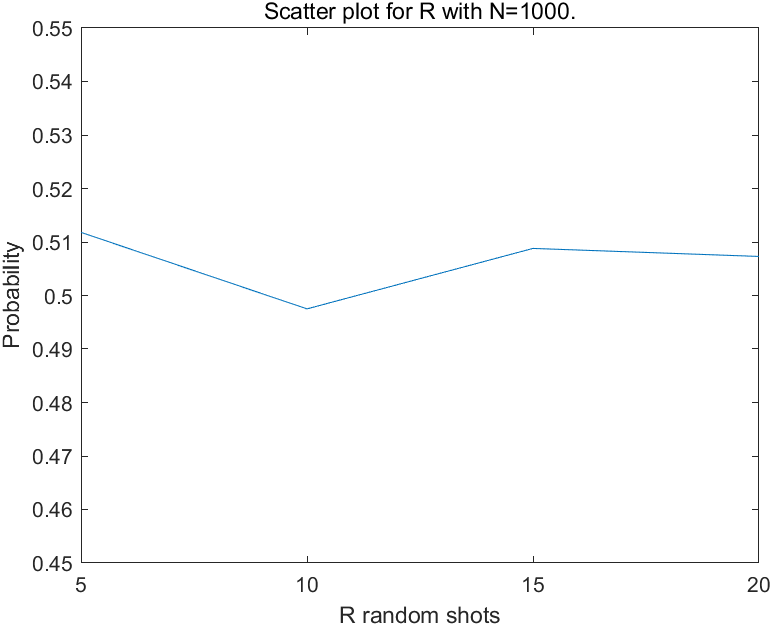
\includegraphics[width=0.5\textwidth]{img/t5.png}
    \caption{Line Chart of Probability against R with N=1000 (Task 5)}
    \label{Fig:task5}
    \end{centering}
\end{figure}

By practicing the source code of Listing \ref{sct5} in Appendix, the probability against R with $N=1000$ was explored. As it shown in Figure \ref{Fig:task5}, similar with the result in Task 4, the probability became stable at 51\% when the experiment repeat more times. However, this phenomenon was not so obvious as it shown in Task4. One reason for this is that the increasing range of Task 4 was around 100000 but the increasing for Task 5 is only 20.

\subsubsection{Task 6: Compare R and N}

From Task4 and Task 5, it was noticed that with the increasing of total shotting times, the probability of scoring would become stable and approach 51.0\%, which is its theoretical value. It was also mentioned that the reason why the tendency of stabilisation in Task 5 was not as obvious as Task 4 was that Task 4 shotting considerably more times than Task 5. In this case, it can also be indicated that the increasing of R and N can both promote the accuracy of the experimental probability.

\subsubsection{Task 7: Gaussian Distribution}


In this case, it was required to substitute the distribution generation method from uniform random distribution to Gaussian random distribution. With a smart design of the program architecture, the only thing needed was to change the method (function) parameters in the code of Task 2\&3, Task 4, Task 5 from unifrnd\_circle to normrnd\_circle.

\begin{figure}[htbp]     \begin{centering}
    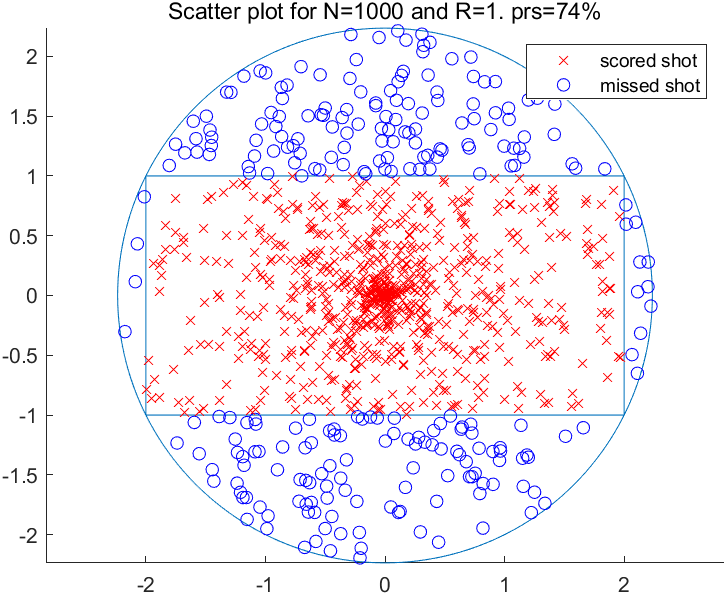
\includegraphics[width=0.5\textwidth]{img/t7_3.png}
    \caption{Shotting Illustration with N=1000 \& R=1 (Task 7\_3)}
    \label{Fig:task7_3}
    \end{centering}
\end{figure}

\newpage

Using the code in Listing \ref{sct7_2}, Task 2 and Task 3 were repeated as required. Figure \ref{Fig:task7_3} illustrated the same simulation with Task 2 with Gaussian method. Comparing with the uniform situation, the distribution in this case seemed to be more centralized at the center of the goal. Inevitably, the probability increased to 74\% in this case, which was considerable large than the uniform one.

\begin{figure}[htbp]     \begin{centering}
    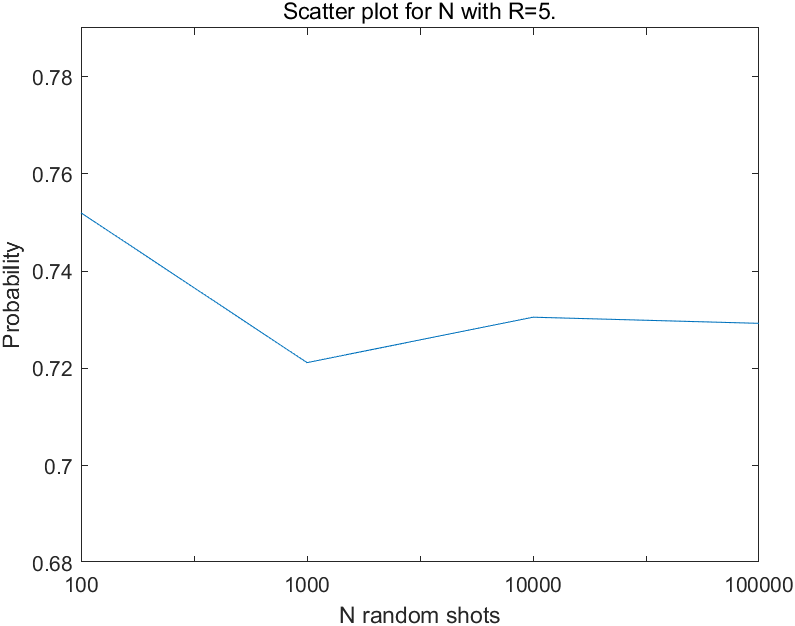
\includegraphics[width=0.5\textwidth]{img/t7_4.png}
    \caption{Line Chart of Probability against N with R=5 (Task 7\_4)}
    \label{Fig:task7_4}
    \end{centering}
\end{figure}

Listing \ref{sct7_4} presented the source code for the repeat of Task 4. By running Listing \ref{sct7_4}, Figure \ref{Fig:task7_4} which explored the relation between scoring probability and shooting times can be generated. Similar with the uniform distribution, with the shotting times increasing, the probability become stable at 73\%, which was different from the value 51\% in uniform case.

\begin{figure}[htbp]     \begin{centering}
    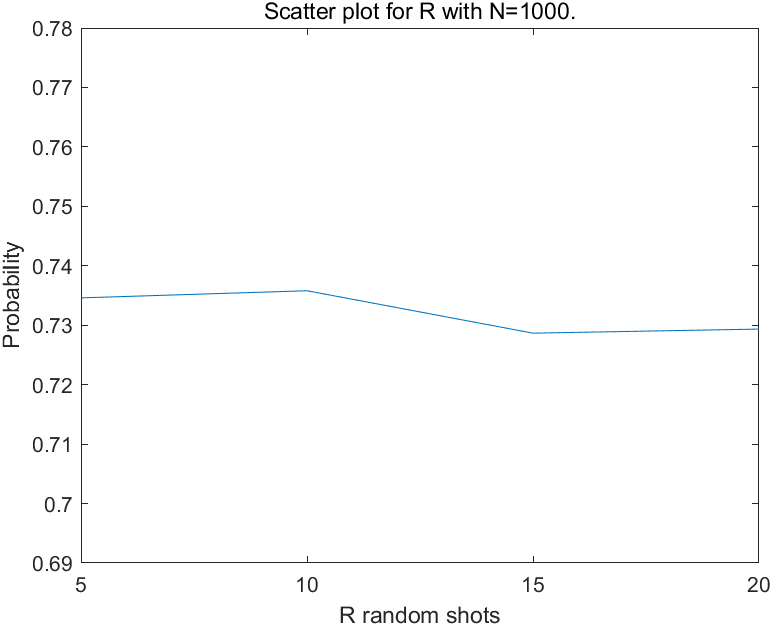
\includegraphics[width=0.5\textwidth]{img/t7_5.png}
    \caption{Line Chart of Probability against R with N=1000 (Task 7\_5)}
    \label{Fig:task7_5}
    \end{centering}
\end{figure}

Listing \ref{sct7_5} displayed the Matlab code for the exploration of the relation between the probability and experiment repeat times R. As the result shown in Figure \ref{Fig:task7_5}, even if the increasing of R was slowly, it can also be figured out that the probability was trying to approach around 73\%.



\subsection{Part 2: With Goalkeeper Tests}

This section presents and comments the result from the simulation with goalkeeper.

\subsubsection{Task 8: Uniform Case}

As the goalkeeper in this case was exist, several functions such as uniform\_5case (Listing \ref{scf:uniform_5case}) was designed to simulate the action of the goalkeeper and one function isGoalKept (Listing \ref{scf:isGoalKept}) was utilized to judge whether a ball was scored. With a Matlab project architecture with high reusability, the addition of goalkeeper can be easily achieved by simply changing several parameters as it shown in Listing \ref{sct8}.


\begin{figure}[htbp]
\centering
\begin{minipage}[t]{0.48\textwidth}
\centering
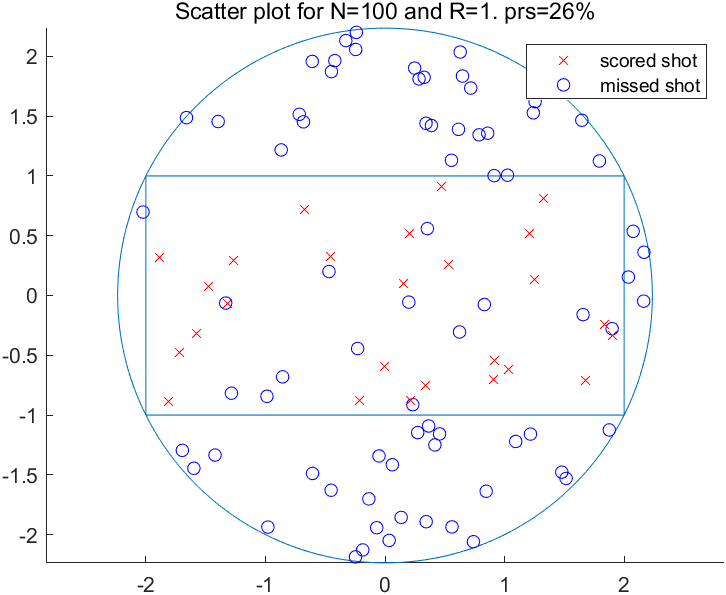
\includegraphics[width=6cm]{img/t8_1.png}
\caption{Scored Balls Distribution Simulation for R=100}
\label{Fig:task8_1}
\end{minipage}
\begin{minipage}[t]{0.48\textwidth}
\centering
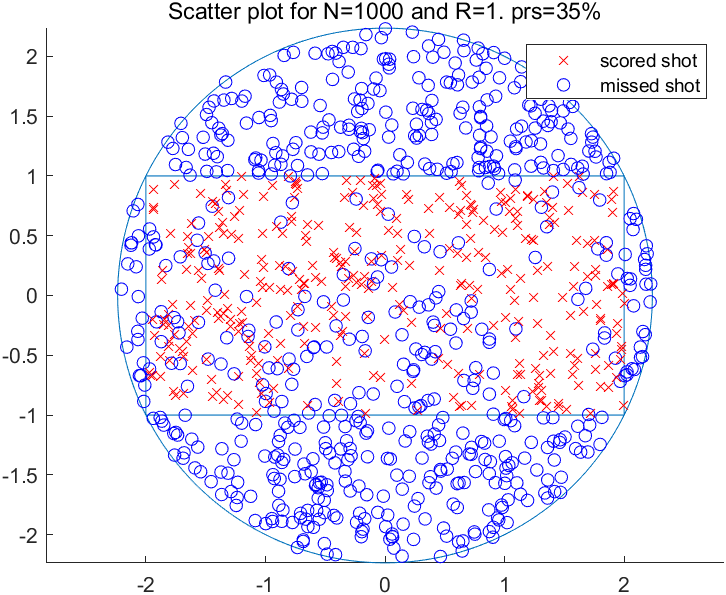
\includegraphics[width=6cm]{img/t8_2.png}
\caption{Scored Balls Distribution Simulation for R=1000}
\label{Fig:task8_2}
\end{minipage}
\end{figure}

Figure \ref{Fig:task8_1} and Figure \ref{Fig:task8_2} displayed the situation of $R=100$ and $R=1000$ correspondingly. It can be noticed that the scoring probability for 100 and 1000 kicks were 26\% and 35\%. After repeating the case of $R=100$ for several times, it was observed that the value of probability was shaken around 35\%, thus it was explained that as the kicks increased, the scoring probability could approach 35\%. Compared with the scoring probability 51\% in Task 1 and Task 3, it can be figured that , with the same distribution method, the scoring probability considerably decreased after adding a goalkeeper.


\subsubsection{Task 9: Gaussian Case}

By substituting the distribution method parameter from Function unifrnd\_circle (Listing \ref{scf:unifrnd_circle}) to Function normrnd\_circle (Listing \ref{scf:normrnd_circle}) as shown in Listing \ref{sct:t9}, the behavior of the kickers can be switched to Gaussian mode.


\begin{figure}[htbp]
\centering
\begin{minipage}[t]{0.48\textwidth}
\centering
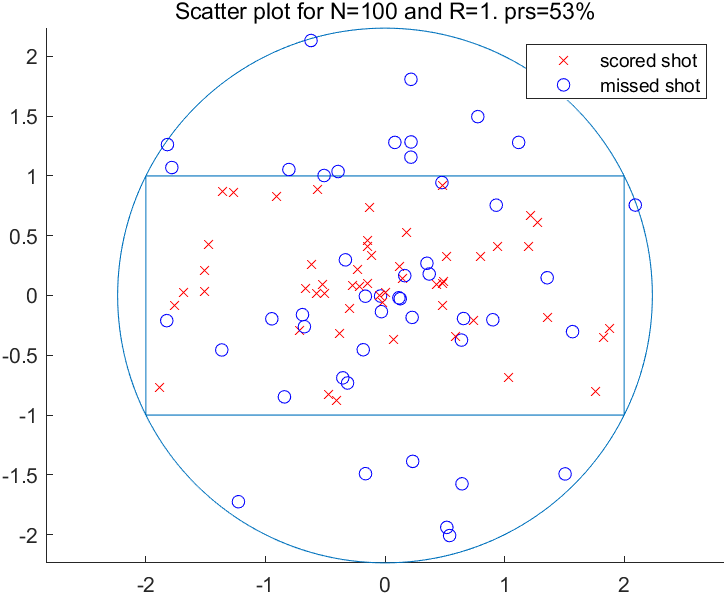
\includegraphics[width=6cm]{img/t9_1.png}
\caption{Scored Balls Distribution (Gaussian) Simulation for R=100}
\label{Fig:task9_1}
\end{minipage}
\begin{minipage}[t]{0.48\textwidth}
\centering
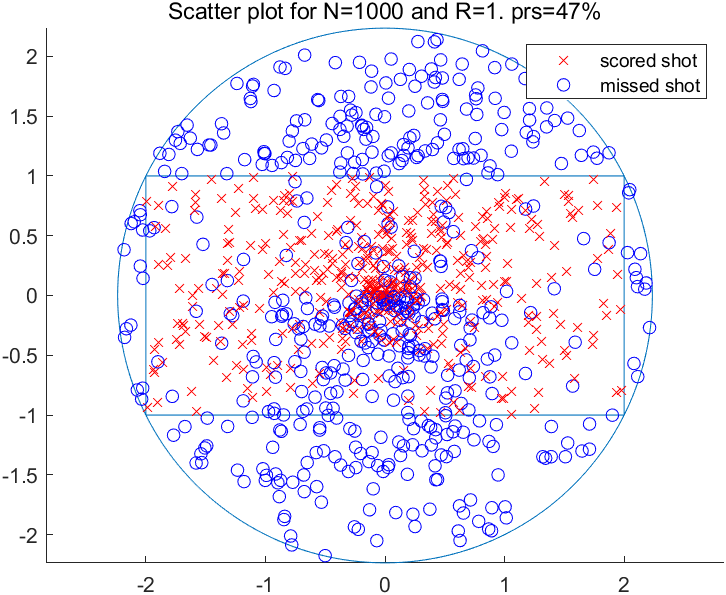
\includegraphics[width=6cm]{img/t9_2.png}
\caption{Scored Balls Distribution (Gaussian) Simulation for R=1000}
\label{Fig:task9_2}
\end{minipage}
\end{figure}

The simulated scoring probability for Gaussian situation was 53\% and 47\% for $R=100$ and $R=1000$ correspondingly. With the increasing of the kicks, the probability approached 47.3\%. The distribution illustrations were shown as Figure \ref{Fig:task9_1} and \ref{Fig:task9_2} respectively. Comparing with the result in Task 8, the concentration of the kicks was higher than the balls distribution in Task 8, which is also the distinct between uniform distribution and Gaussian distribution. Therefore, the final scoring probability was improved as more kicks fallen into the goal. Different from the result in Task 7 with no goalkeeper, the scoring probability was considerable decreased since a considerable number of kicks in the goal were blocked by the goalkeeper. This explained the drop down of the result from Task 7 to this Task.


\subsubsection{Task 10: Smarter Goalkeepers}

In this part, the goalkeeper was required to be simulated to be smarter. For technique reasons, it was assumed that the goalkeeper tended to choose the last two cases in Figure \ref{Fig:goalkeeper-action} with 90\%. To achieve this, a uniform\_5case\_plus (Listing \ref{scf:uniform_5case_plus}) Function was designed to substitute the former uniform\_5case (Listing \ref{scf:uniform_5case}) Function to Listing \ref{sct:t10_8} and Listing \ref{sct:t10_9}. After the modification, the result can be generated with Function unifrnd\_circle (Listing \ref{scf:unifrnd_circle}) in uniform case and Function normrnd\_circle (Listing \ref{scf:normrnd_circle}) in Gaussian case.


\begin{figure}[htbp]
\centering
\begin{minipage}[t]{0.48\textwidth}
\centering
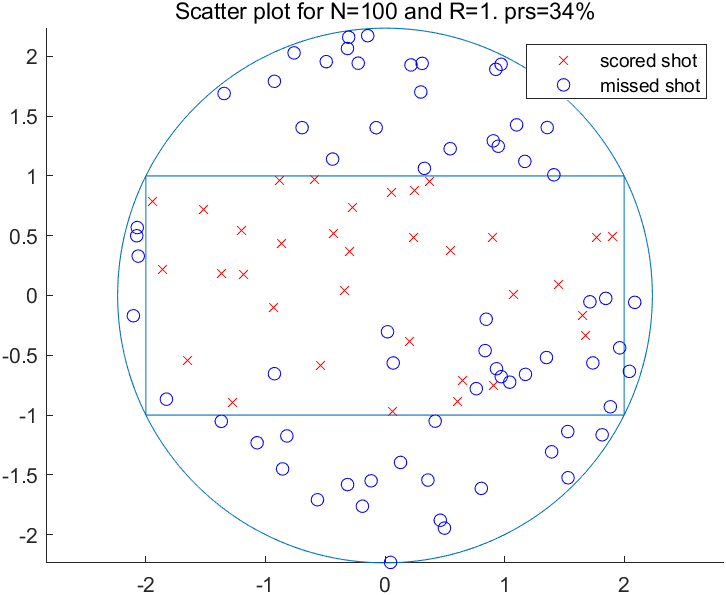
\includegraphics[width=6cm]{img/t10_11.png}
\caption{Scored Balls Distribution Simulation for R=100}
\label{Fig:task10_11}
\end{minipage}
\begin{minipage}[t]{0.48\textwidth}
\centering
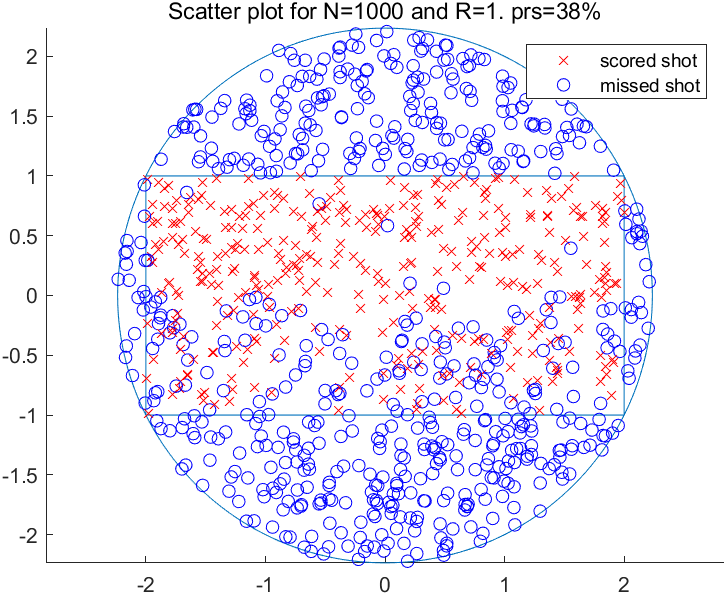
\includegraphics[width=6cm]{img/t10_12.png}
\caption{Scored Balls Distribution Simulation for R=1000}
\label{Fig:task10_12}
\end{minipage}
\end{figure}

\newpage

Figure \ref{Fig:task10_11} and Figure \ref{Fig:task10_12} presented the result of 100 kicks and 1000 kicks with uniform distribution, which were 37\% and 38\% correspondingly. Comparing with the result 26\% and 35\% in Task 8, it was observed that the scoring probability was increased since the goalkeeper only tended to block the kicks in the 4\&5 cases, which may mean that there were more scored kicks on the upper and middle area.

\begin{figure}[htbp]
\centering
\begin{minipage}[t]{0.48\textwidth}
\centering
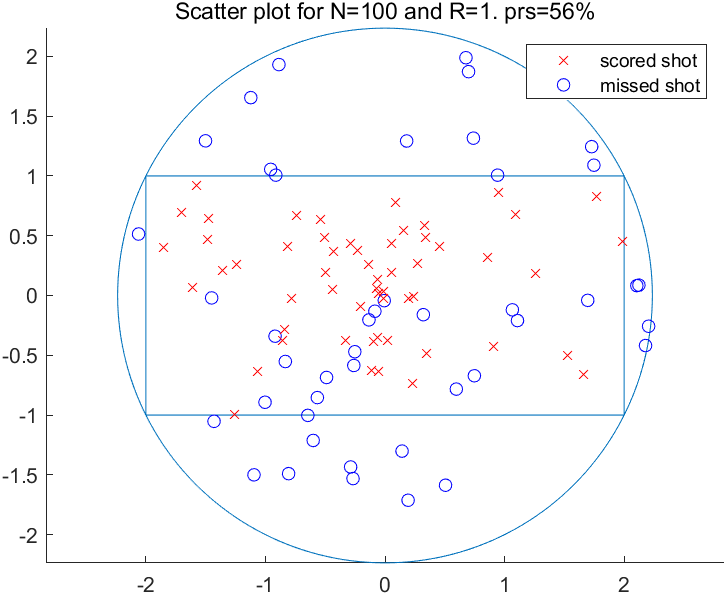
\includegraphics[width=6cm]{img/t10_21.png}
\caption{Scored Balls Distribution (Gaussian) Simulation for R=100}
\label{Fig:task10_21}
\end{minipage}
\begin{minipage}[t]{0.48\textwidth}
\centering
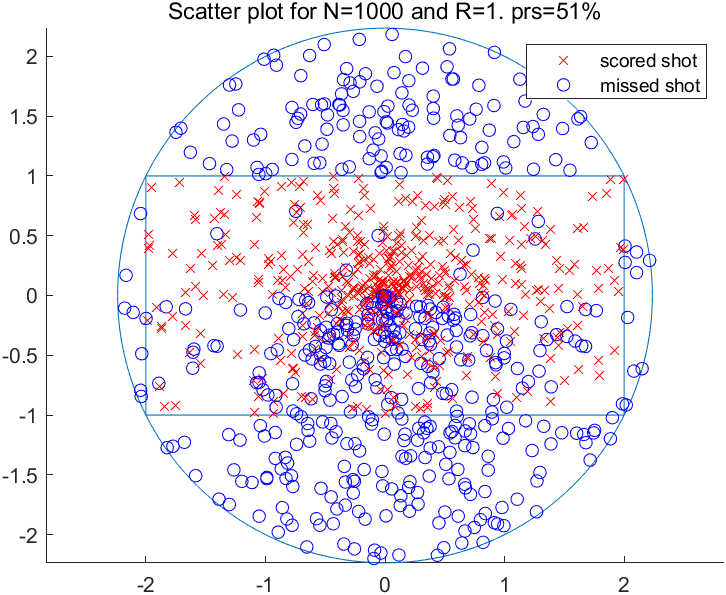
\includegraphics[width=6cm]{img/t10_22.png}
\caption{Scored Balls Distribution (Gaussian) Simulation for R=1000}
\label{Fig:task10_22}
\end{minipage}
\end{figure}

Figure \ref{Fig:task10_21} and Figure \ref{Fig:task10_22} displayed the Gaussian method simulation result with the kicks of 100 and 1000, which were 56\% and 51\%. Unlike to the result 53\% and 47\% in Task 9, it can also be indicated that the scoring probability was decreased comparing to the situation that the goalkeeper uniformly randomly acted. The reason for this was considered quite similar to the reason mentioned in the last paragraph. Nevertheless, the result should be slight different as the distribution was changed to Gaussian distribution thus this could give rise to a distinct increased value of the final result, which was not clearly indicated by the simulation.


%------------------------------------------------------------------------------------------------------- 
\section{Discussion}
%-------------------------------------------------------------------------------------------------------

In terms of the advantages of Monte Carlo method, from this experiment, four advantages can be concluded. Firstly, with Monte Carlo method, a complex math process, such as the calculation of the scoring probability in Gaussian distribution, can be easily achieved through a computer. Secondly, with the increasing of the experiment repeat times, the error of the result can be considerably reduced. Furthermore, it was flexible when using Monte Carlo method to balance the accuracy of the result and the time consumed on computing, which means that, it would be possible to obtain a rough result in a short time in some situation. Additionally, nearly all problems which can be transformed to statistic problems can be approached via Monte Carlo method. \textbf{Q1}

The drawbacks of Monte Carlo method were mainly classified into the following three points. Firstly, a considerable number of computing resources and time are required when using Monte Carlo method to obtain a accuracy result. Secondly, the error generated by the Monte Carlo method is probability error and can not be effectively removed. Moreover, as the generation process is simulated artificially, Monte Carlo method seems to be limited in some periodical application and may give rise to generate same random values. \textbf{Q1}

Although the model in this experiment has fully considered the situation of the kicks and the actions of the goalkeeper, there are still several improvement can be proposed. Firstly, the reaction of the goalkeeper could be designed according to the kicking direction of the kicker. Secondly, the effect from the environment such as the wind and the sun, which may dazzling the goalkeeper, can also be considered and influence the action of the kickers and the goal keeper. Besides, the behavior classification of the goalkeeper can be further divided. Furthermore, it is also believed that even the goalkeeper choose the right action, it is still possible that the ball finally go through the goal and scores. \textbf{Q2}

After changing the standard deviation of the Gaussian distribution in Task 7 and Task 9, it was observed that the result of scoring probability would change. For both Task 7 and Task 8, when the standard deviation become smaller, the kicks will become more concentrated to the center of the goal, which indicates increasing precision and not changing accuracy. \textbf{Q3}

To find the relation of estimating the value of $\pi$, from Equation \ref{eq:posibility_by_area}, the following Equation can be obtained. \textbf{Q4}.

\begin{equation}
P_{scoring} = \frac{WL}{\pi R^2}.
\label{eq:P_detail}
\end{equation}

From Equation \ref{eq:P_detail}, the relation of $\pi$ and $P_{scoring}$ can be conducted as the following equation.

\begin{equation}
\pi = \frac{WL}{P_{scoring} R^2}.
\label{eq:estimate_pi}
\end{equation}

After input the result of scoring probability 51\% in Task 2 to Equation \ref{eq:estimate_pi}, the value of $\pi$ can be calculated, which is $3.137$. For the result in the Gaussian case, after the value 74\% is input, the $\pi$ is calculated to be $2.16$, which is quite far from the right value. The reason for this is that the area of the circle which contains the $\pi$ is formed uniformly, which is similar to the definition of uniform distribution but different from the Gaussian distribution. In a word, the ununiformity of Gaussian distribution causes this deviation. \textbf{Q4}

From the result of Part 2 simulation (Figure \ref{Fig:task8_2}, \ref{Fig:task9_2}, \ref{Fig:task10_12}, \ref{Fig:task10_22}), it is advised to the penalty takers that the scoring opportunity could be higher if they kick towards the upper left corner and upper right corner. As for the goalkeepers, it is suggested that they should protect the corner of the goal more and not just focus on several special action modes, which means that, try to protect the area of the goal as much as possible. \textbf{Q5}

%-------------------------------------------------------------------------------------------------------
\section{Conclusions}
%-------------------------------------------------------------------------------------------------------

In this experiment, features and application of Monte Carlo method were explored and discussed with the assistance of Matlab. Penalty kicks were simulated with the distribution of kicks following uniform distribution and Gaussian distribution and the goalkeeper with different behaviors. It was further discussed about the advantages and limitation of Monte Carlo method as well as some suggestions against the penalty takers and the goalkeepers on the basis of the modeling result.

%

%-------------------------------------------------------------------------------------------------------

\bibliographystyle{IEEEtran}
\bibliography{MyRefs}         % The file MyRefs.bib contains the actual bibliography material
                                  % References section created automatically
\addcontentsline{toc}{section}{References}



% --------------------------- This is how to declare the Appendices section ----------------------------
\newpage
\appendix
\appendixpage
\addappheadtotoc


%-------------------------------------------------------------------------------------------------------
\section{Matlab Source Code}
%-------------------------------------------------------------------------------------------------------

\subsection{Overall Structure}

This is the source code files structure instruction, which displays the list of main code files and function files.

\lstset{language=MATLAB, frame=single, basicstyle=\footnotesize, backgroundcolor=\color{MyLightYellow}, caption={Source Code Files Structure},label=Listing:tree}
\lstinputlisting[language=MATLAB]{../src/tree.js}


\subsection{Main Codes}

\subsubsection{Task 2\&3}

%-------------------------- Source code / program listings can be inserted using like this -----------
\lstset{language=MATLAB, frame=single, basicstyle=\footnotesize, backgroundcolor=\color{MyLightYellow}, caption={Matlab Source Code for Task 2},label=sct2}
\lstinputlisting[language=MATLAB]{../src/t2.m}
%-------------------------------------------------------------------------------------------------------


\subsubsection{Task 4}

%-------------------------- Source code / program listings can be inserted using like this -----------
\lstset{language=MATLAB, frame=single, basicstyle=\footnotesize, backgroundcolor=\color{MyLightYellow}, caption={Matlab Source Code for Task 4},label=sct4}
\lstinputlisting[language=MATLAB]{../src/t4.m}
%-------------------------------------------------------------------------------------------------------


\subsubsection{Task 5}

%-------------------------- Source code / program listings can be inserted using like this -----------
\lstset{language=MATLAB, frame=single, basicstyle=\footnotesize, backgroundcolor=\color{MyLightYellow}, caption={Matlab Source Code for Task 5},label=sct5}
\lstinputlisting[language=MATLAB]{../src/t5.m}
%-------------------------------------------------------------------------------------------------------


\subsubsection{Task 7}

%-------------------------- Source code / program listings can be inserted using like this -----------
\lstset{language=MATLAB, frame=single, basicstyle=\footnotesize, backgroundcolor=\color{MyLightYellow}, caption={Matlab Source Code for Task 7\_2},label=sct7_2}
\lstinputlisting[language=MATLAB]{../src/t7_2.m}
%-------------------------------------------------------------------------------------------------------

%-------------------------- Source code / program listings can be inserted using like this -----------
\lstset{language=MATLAB, frame=single, basicstyle=\footnotesize, backgroundcolor=\color{MyLightYellow}, caption={Matlab Source Code for Task 7\_4},label=sct7_4}
\lstinputlisting[language=MATLAB]{../src/t7_4.m}
%-------------------------------------------------------------------------------------------------------

%-------------------------- Source code / program listings can be inserted using like this -----------
\lstset{language=MATLAB, frame=single, basicstyle=\footnotesize, backgroundcolor=\color{MyLightYellow}, caption={Matlab Source Code for Task 7\_5},label=sct7_5}
\lstinputlisting[language=MATLAB]{../src/t7_5.m}
%-------------------------------------------------------------------------------------------------------

\subsubsection{Task 8}

%-------------------------- Source code / program listings can be inserted using like this -----------
\lstset{language=MATLAB, frame=single, basicstyle=\footnotesize, backgroundcolor=\color{MyLightYellow}, caption={Matlab Source Code for Task 8},label=sct8}
\lstinputlisting[language=MATLAB]{../src/t8.m}
%-------------------------------------------------------------------------------------------------------

\subsubsection{Task 9}

%-------------------------- Source code / program listings can be inserted using like this -----------
\lstset{language=MATLAB, frame=single, basicstyle=\footnotesize, backgroundcolor=\color{MyLightYellow}, caption={Matlab Source Code for Task 9},label=sct9}
\lstinputlisting[language=MATLAB]{../src/t9.m}
%-------------------------------------------------------------------------------------------------------

\subsubsection{Task 10}

%-------------------------- Source code / program listings can be inserted using like this -----------
\lstset{language=MATLAB, frame=single, basicstyle=\footnotesize, backgroundcolor=\color{MyLightYellow}, caption={Matlab Source Code for Task 10\_8},label=sct10_8}
\lstinputlisting[language=MATLAB]{../src/t10_8.m}
%-------------------------------------------------------------------------------------------------------


%-------------------------- Source code / program listings can be inserted using like this -----------
\lstset{language=MATLAB, frame=single, basicstyle=\footnotesize, backgroundcolor=\color{MyLightYellow}, caption={Matlab Source Code for Task 10\_9},label=sct10_9}
\lstinputlisting[language=MATLAB]{../src/t10_9.m}
%-------------------------------------------------------------------------------------------------------

\subsection{Function Codes}

\subsubsection{Draw}

%-------------------------- Source code / program listings can be inserted using like this -----------
\lstset{language=MATLAB, frame=single, basicstyle=\footnotesize, backgroundcolor=\color{MyLightYellow}, caption={Matlab Source Code for Function drawBackGround},label=scf:drawBackGround}
\lstinputlisting[language=MATLAB]{../src/func/drawBackGround.m}
%-------------------------------------------------------------------------------------------------------

\subsubsection{Math}

%-------------------------- Source code / program listings can be inserted using like this -----------
\lstset{language=MATLAB, frame=single, basicstyle=\footnotesize, backgroundcolor=\color{MyLightYellow}, caption={Matlab Source Code for Function getDisProb},label=scf:getDisProb}
\lstinputlisting[language=MATLAB]{../src/func/getDisProb.m}
%-------------------------------------------------------------------------------------------------------

\subsubsection{Tools}

%-------------------------- Source code / program listings can be inserted using like this -----------
\lstset{language=MATLAB, frame=single, basicstyle=\footnotesize, backgroundcolor=\color{MyLightYellow}, caption={Matlab Source Code for Function getDisProb},label=scf:getDisProb}
\lstinputlisting[language=MATLAB]{../src/func/getDivByPos.m}
%-------------------------------------------------------------------------------------------------------

%-------------------------- Source code / program listings can be inserted using like this -----------
\lstset{language=MATLAB, frame=single, basicstyle=\footnotesize, backgroundcolor=\color{MyLightYellow}, caption={Matlab Source Code for Function isGoalKept},label=scf:isGoalKept}
\lstinputlisting[language=MATLAB]{../src/func/isGoalKept.m}
%-------------------------------------------------------------------------------------------------------

%-------------------------- Source code / program listings can be inserted using like this -----------
\lstset{language=MATLAB, frame=single, basicstyle=\footnotesize, backgroundcolor=\color{MyLightYellow}, caption={Matlab Source Code for Function isInRect},label=scf:isInRect}
\lstinputlisting[language=MATLAB]{../src/func/isInRect.m}
%-------------------------------------------------------------------------------------------------------


\subsubsection{Distribution Methods}

%-------------------------- Source code / program listings can be inserted using like this -----------
\lstset{language=MATLAB, frame=single, basicstyle=\footnotesize, backgroundcolor=\color{MyLightYellow}, caption={Matlab Source Code for Function normrnd\_circle},label=scf:normrnd_circle}
\lstinputlisting[language=MATLAB]{../src/func/normrnd_circle.m}
%-------------------------------------------------------------------------------------------------------

%-------------------------- Source code / program listings can be inserted using like this -----------
\lstset{language=MATLAB, frame=single, basicstyle=\footnotesize, backgroundcolor=\color{MyLightYellow}, caption={Matlab Source Code for Function uniform\_5case},label=scf:uniform_5case}
\lstinputlisting[language=MATLAB]{../src/func/uniform_5case.m}
%-------------------------------------------------------------------------------------------------------

%-------------------------- Source code / program listings can be inserted using like this -----------
\lstset{language=MATLAB, frame=single, basicstyle=\footnotesize, backgroundcolor=\color{MyLightYellow}, caption={Matlab Source Code for Function uniform\_5case\_plus},label=scf:uniform_5case_plus}
\lstinputlisting[language=MATLAB]{../src/func/uniform_5case_plus.m}
%-------------------------------------------------------------------------------------------------------


%-------------------------- Source code / program listings can be inserted using like this -----------
\lstset{language=MATLAB, frame=single, basicstyle=\footnotesize, backgroundcolor=\color{MyLightYellow}, caption={Matlab Source Code for Function unifrnd\_circle},label=scf:unifrnd_circle}
\lstinputlisting[language=MATLAB]{../src/func/unifrnd_circle.m}
%-------------------------------------------------------------------------------------------------------



\end{document}
